% !TEX root = main.tex

\section{Numerical Results}\label{sec:results}
  \subsection{Manufactured Solution}\label{ssec:manufactured_solution}
    In order to confirm the order of accuracy of our method, we use the method of
    manufactured solutions.
    The method of manufactured solutions picks an exact solution \(\hat{q}\) and then adds
    a source term to the initial partial differential equation to make \(\hat{q}\) the
    true solution to the new differential equation.
    So we actually solve
    \begin{equation}
        q_t + \p{q^2 - q^3}_x = -\p{q^3 q_{xxx}}_x + s,
    \end{equation}
    where
    \begin{equation}
        s = \hat{q}_t + \p{\hat{q}^2 - \hat{q}^3}_x + \p{\hat{q}^3 \hat{q}_{xxx}}_x.\label{eq:source_term}
    \end{equation}
    This new PDE's exact solution is now \(\hat{q}\).
    We chose
    \begin{equation}
        \hat{q} = 0.1 \times \sin{2 \pi / 20.0 \times (x - t)} + 0.15,\label{eq:exact_solution}
    \end{equation}
    on \(x \in \br{0, 40}\) with periodic boundary conditions to be our manufactured
    solution.
    This manufactued solution is chosen so that our flux \(q^2 - q^3\) is in it's convex
    region.

    We solve this problem until \(t = 5.0\) with constant, linear, and quadratic basis
    polynomials.
    The time step size for these simulations is determined by the
    Courant–Friedrichs–Lewy (CFL) condition.
    The CFL condition states that
    \begin{equation}
      \Delta t = \nu \frac{\Delta x}{\lambda},
    \end{equation}
    where \(\lambda \) is the wavespeed and \(\nu \) is the CFL number.
    For hyperbolic problems solved with explicit Runge-Kutta time-stepping, \(\nu \),
    typically follows the pattern \(\frac{1}{2n - 1} \) where \(n\) is the order of the
    method.
    For this example the wavespeed is \(1\), and the timestep is chosen just smaller
    then the typical CFL number.
    Specifically the timesteps were \(\Delta t = 0.9 \Delta x\),
    \(\Delta t = 0.2 \Delta x\), and \(\Delta t = 0.1 \Delta x\)
    for first, second and third order respectively.

    Table~\ref{tab:convergence_results} shows the error for each simulation as the mesh
    is refined.
    The table also shows the rate of convergence to the true solution, and in each case
    the rate of convergence approaches the expected order.
    Note that the first, second, and third order methods only require one Picard
    iteration to converge at the expected order.

    The relative \(L^2\) error is defined as
    \begin{equation}
      E = \norm[L^2(a, b)]{e(x)} = \sqrt{\frac{\dintt{a}{b}{\p{\hat{q} - q_h}^2}{x}}{\dintt{a}{b}{\hat{q}^2}{x}}} \label{eq:l2_error}
    \end{equation}
    Since we are using an orthonormal basis of \(V_h^k\), there is an easier way to
    compute this error numerically.
    The basis consists of functions \(\phi_j^l\), that are polynomials of degree \(l\)
    on \(I_j\) and are zero everywhere else for \(j = 1, \ldots, N\) and
    \(l = 0, \ldots, k\).
    By definition of orthonormality we have that
    \begin{equation}
      \dintt{a}{b}{\phi_i^k \phi_j^l}{x} = \delta_{kl} \delta_{ij}
    \end{equation}
    where \(\delta \) is the Kronecker delta.
    In other words on cell \(I_j\), \(\phi_j^l\) is a Legendre polynomial.
    Given this basis we can express our numerical solution, \(q_h \in V_h^k\), as
    \begin{equation}
      \eval{q_h}{I_j} = \sum{l = 0}{k}{Q_j^l \phi_j^l},
    \end{equation}
    for all \(j\), where \(Q_j^l\) are constant coefficients.

    In order to maintain leading order accuracy we project our exact solution,
    \(\hat{q}\), onto the space \(V_h^{k+1}\).
    Let \(\hat{q}_h\) denote this projection.
    We use the same orthonormal basis with the addition of \(\phi_j^{k+1}\) on each
    cell.
    In this case we have the following representation
    \begin{equation}
      \eval{\hat{q}_h}{I_j} = \sum{l = 0}{k+1}{\hat{Q}_j^l \phi_j^l(x)} \text{ and }
      \eval{q_h}{I_j} = \sum{l = 0}{k+1}{Q_j^l \phi_j^l(x)}.
    \end{equation}
    where \(Q_j^{k+1}\) will be zero.
    Substituting these representations into the \(L^2\) error, equation~\eqref{eq:l2_error},
    and using the orthonormality property gives the following expression for the error,
    \begin{equation}
      E_N = \sqrt{\frac{\sum*{j = 1}{N}{\sum*{l = 0}{k+1}{\p{\hat{Q}_i - Q_i}^2}}}{\sum{j=1}{N}{\sum{l=0}{k+1}{\hat{Q}_i^2}}}}.
    \end{equation}
    This expression is equivalent to equation~\eqref{eq:l2_error} to leading order.
    The order of convergence is then estimated from these errors as
    \begin{equation}
      \text{order} \approx \log[2]{\frac{E_N}{E_{2N}}}.
    \end{equation}

    \begin{table}
      \centering
      \begin{tabular}{r*{6}l}
        \toprule
        & \multicolumn{2}{c}{1st Order} & \multicolumn{2}{c}{2nd Order} & \multicolumn{2}{c}{3rd Order} \\
        \midrule
        \(n\) & \multicolumn{1}{c}{error} & order & \multicolumn{1}{c}{error} & order & \multicolumn{1}{c}{error} & order\\
        \midrule
          20 &   \(0.136\) &  --- & \(7.33 \times 10^{-3}\) &  --- & \(5.29 \times 10^{-4}\) &  --- \\
          40 &  \(0.0719\) & 0.92 & \(1.99 \times 10^{-3}\) & 1.88 & \(5.38 \times 10^{-5}\) & 3.30 \\
          80 &  \(0.0378\) & 0.93 & \(5.60 \times 10^{-4}\) & 1.83 & \(7.47 \times 10^{-6}\) & 2.85 \\
         160 &  \(0.0191\) & 0.99 & \(1.56 \times 10^{-4}\) & 1.85 & \(9.97 \times 10^{-7}\) & 2.91 \\
         320 & \(0.00961\) & 0.99 & \(3.98 \times 10^{-5}\) & 1.97 & \(1.26 \times 10^{-7}\) & 2.98 \\
         640 & \(0.00483\) & 0.99 & \(1.00 \times 10^{-5}\) & 1.99 & \(1.58 \times 10^{-8}\) & 3.00 \\
        1280 & \(0.00242\) & 1.00 & \(2.50 \times 10^{-6}\) & 2.00 & \(1.98 \times 10^{-9}\) & 3.00 \\
        \bottomrule
      \end{tabular}
      \caption{Convergence table with a constant, linear, quadratic polynomial bases.
      CFL = 0.9, 0.2, 0.1 respectively.}\label{tab:convergence_results}
    \end{table}
    % Table~\ref{tab:iteration_results} shows how the error is affected when the number of
    % Picard iterations is decreased.

    % \begin{table}
    %   \centering
    %   \begin{tabular}{r*{6}l}
    %     \toprule
    %          & \multicolumn{2}{c}{1 Iteration} & \multicolumn{2}{c}{2 Iterations} & \multicolumn{2}{c}{3 Iterations} \\
    %     \midrule
    %     \(n\)& \multicolumn{1}{c}{error} & order & \multicolumn{1}{c}{error} & order & \multicolumn{1}{c}{error} & order\\
    %     \midrule
    %       20 & & & & & \(5.29 \times 10^{-4}\) & --- \\
    %       40 & & & & & \(5.38 \times 10^{-5}\) & 3.30 \\
    %       80 & & & & & \(7.47 \times 10^{-6}\) & 2.85 \\
    %      160 & & & & & \(9.97 \times 10^{-7}\) & 2.91 \\
    %      320 & & & & & \(1.26 \times 10^{-7}\) & 2.98 \\
    %      640 & & & & & \(1.58 \times 10^{-8}\) & 3.00 \\
    %     \bottomrule
    %   \end{tabular}
    %   \caption{Convergence table with a quadratic polynomial basis. One, Two, and Three
    %   Picard iterations are used for each nonlinear solve. CFL = 0.1}\label{tab:iteration_results}
    % \end{table}

\subsection{Traveling Waves}\label{ssec:bertozzi_cases}
  In this section we showcase several numerical examples that demonstrate the traveling
  wave profiles of equation~\eqref{eq:thin_film_model}.
  The traveling wave profiles differ from the standard hyperbolic wave profile in
  several ways.
  They differ in that they may not be unique and may include undercompressive shocks.
  These examples were first shown in~\cite{article:Bertozzi1999} with first order accuracy.
  We now show these examples with our third order method with one Picard iteration and
  a CFL number of \(0.1\).

  In these examples, we use a moving reference frame to keep the mesh size reasonable.
  This is done by actually simulating the following equation,
  \begin{equation}
    q_t + \p{q^2 - q^3 - sq}_x = -\p{q^3 q_{xxx}}_x \label{eq:thin_film_moving_reference_frame}
  \end{equation}
  where \(s\) is the Rankine-Hugoniot wavespeed of the original numerical flux, \(f\)
  \begin{equation}
    s = \frac{f(q_l) - f(q_r)}{q_l - q_r} = q_l + q_r - (q_l^2 + q_l q_r + q_r^2).\label{eq:ranking_hugoniot}
  \end{equation}
  This modified equation will have zero wavespeed in most cases and simulates the
  original PDE in a moving reference frame.

  These examples consider Riemann Problems with different left and right states.
  Depending on the left and right states they are several different wave profiles.
  For these examples we will fix the right state and vary the left state.
  The wave profiles would be qualitatively equivalent for different values for the right
  state, however the values of the left state would also need to change accordingly.

  \subsubsection{Case 1: Unique Weak Lax Shock}\label{sssec:case1}
    Consider a Riemann Problem with left state, \(q_l = 0.3\), and right state,
    \(q_r = 0.1\).
    We will use the following smoothed out profile as an initial condition for this
    problem
    \begin{equation}
      q_0(x) = \p{\tanh{-x} + 1} \frac{q_l - q_r}{2} + q_r.
    \end{equation}
    For this initial condition the numerical solution approaches a steady wave profile
    with a unique Lax type shock.
    Figure~\ref{fig:case1} shows a plot of the solution with this initial condition after
    enough time for the solution to hit its steady state.
    Note that this behavior persists for all \(q_l\) up to some bound which depends on
    \(q_r\).
    \begin{figure}
      \centering
      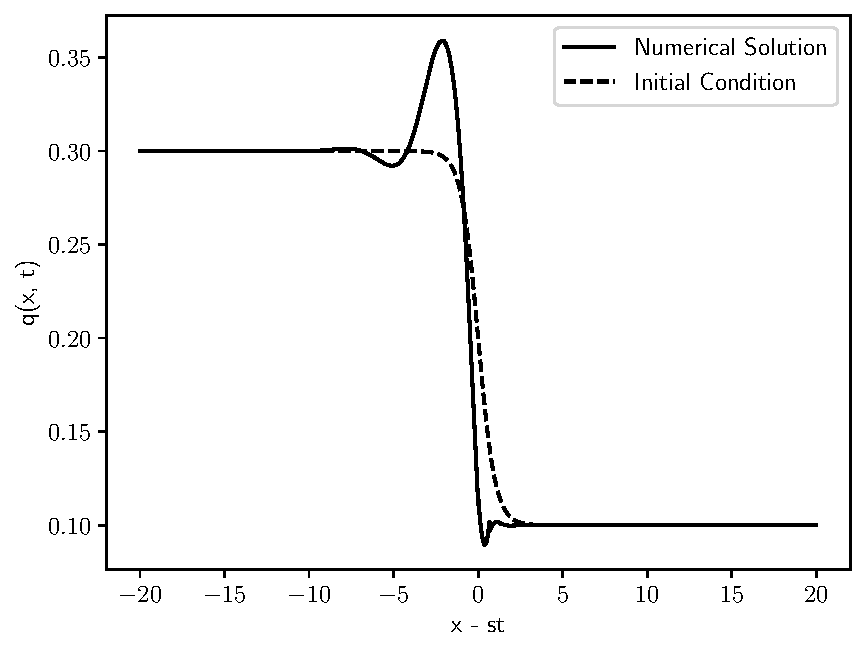
\includegraphics[scale=0.5]{figures/case_1_1.pdf}
      \caption{Case 1: Unique Lax Shock.}\label{fig:case1}
    \end{figure}

  \subsubsection{Case 2: Multiple Lax Shocks}\label{sssec:case2}
    If the left state is increased to \(q_l = 0.3323\), then the wave profile is no
    longer unique.
    In this case the steady traveling wave depends on the initial conditions.

    For the following initial conditions,
    \begin{equation}
      q_0(x) = \p{\tanh{-x} + 1} \frac{q_l - q_r}{2} + q_r, \label{eq:case2_1}
    \end{equation}
    the behavior is the same as in case 1.
    The numerical solution for this initial condition is shown in Figure~\ref{fig:case2}

    Now consider the following initial conditions,
    \begin{equation}
      q_0(x) =
      \begin{cases}
        \p{\p{0.6 - q_l}/2} \tanh{x} + \p{\p{0.6 + q_l}/2} & x < 5 \\
        -\p{\p{0.6 - q_r}/2} \tanh{x - 10} + \p{\p{0.6 + q_r}/2} & x > 5
      \end{cases}.\label{eq:case2_2}
    \end{equation}
    The reader might expect this initial condition to approach the traveling wave shown
    earlier as it has the same far field boundary values, however this is not the case.
    The traveling wave profile that is approaches is shown in Figure~\ref{fig:case2}.

    \begin{figure}
      \centering
      \begin{tabular}{cc}
      (a)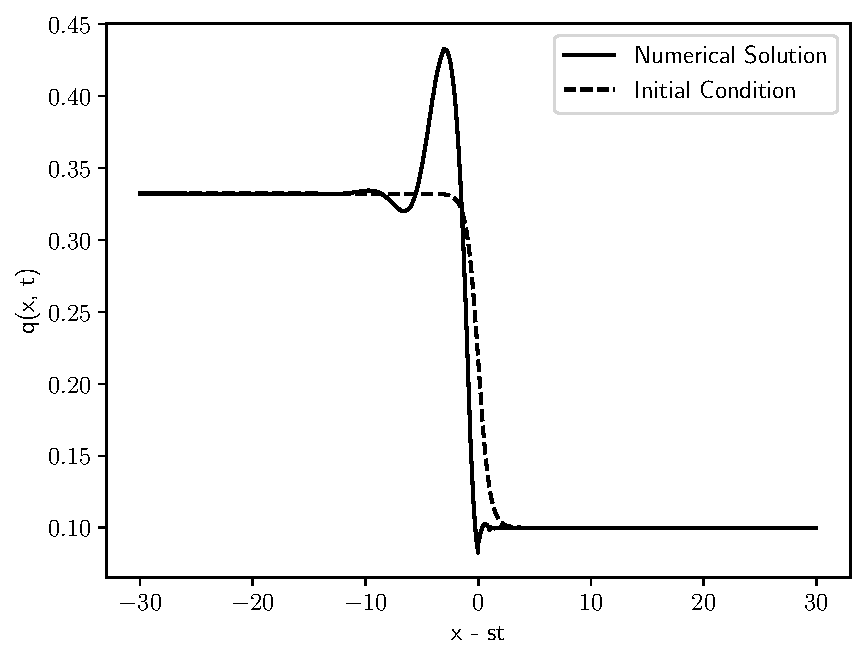
\includegraphics[scale=0.35]{figures/case_2_1.pdf} &
      (b)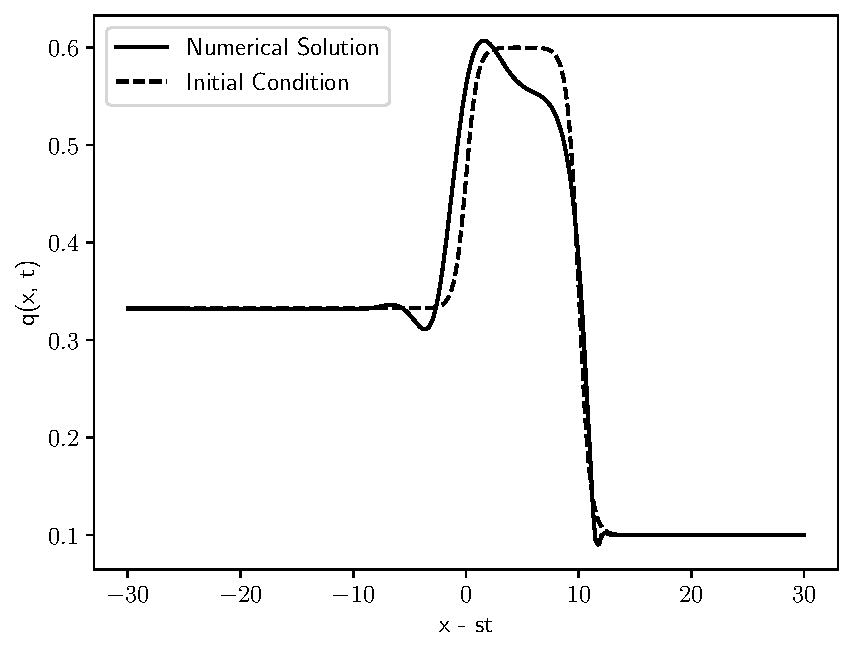
\includegraphics[scale=0.35]{figures/case_2_2.pdf} \\
      \multicolumn{2}{c}{(c)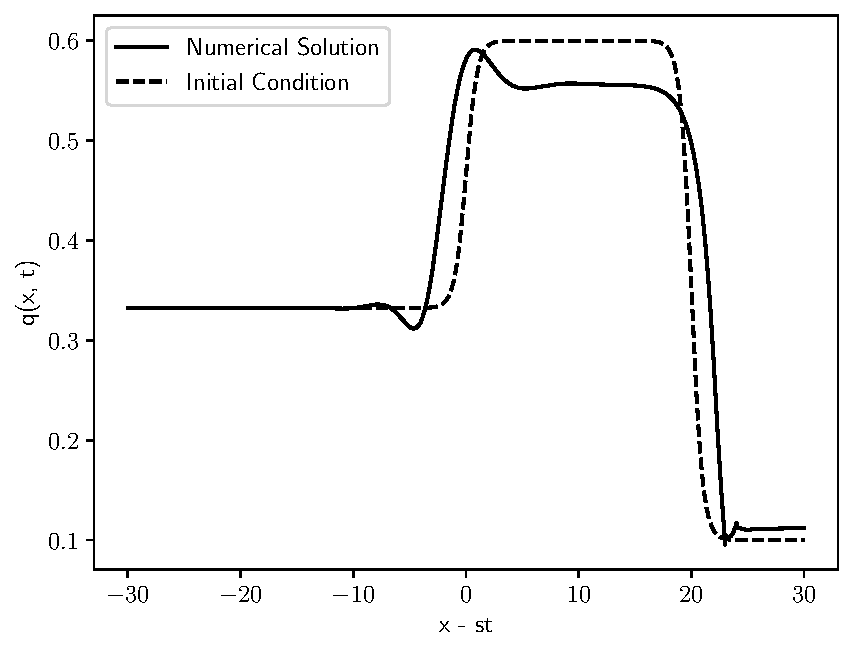
\includegraphics[scale=0.35]{figures/case_2_3.pdf}}
      \end{tabular}
      \caption{Case 2: Distinct Lax Shocks. Panels (a) and (b) show two distinct
      steady travelling waves formed from different initial conditions.
      Panel (c) shows an unsteady wave with a double shock structure from a third
      initial condition.}\label{fig:case2}
    \end{figure}

    These are not the only possible wave profiles possible with these left and right
    states.
    Figure~\ref{fig:case2} part (c) shows the result for the following initial condition,
    \begin{equation}
      q_0(x) =
      \begin{cases}
        \p{\p{0.6 - q_l}/2} \tanh{x} + \p{\p{0.6 + q_l}/2} & x < 10 \\
        -\p{\p{0.6 - q_r}/2} \tanh{x - 20} + \p{\p{0.6 + q_r}/2} & x > 10
      \end{cases}\label{eq:case2_3}.
    \end{equation}
    This initial condition has a larger hump then equation~\eqref{eq:case2_2}, and the
    traveling wave reflects this aspect.
    In this case the traveling wave is not a steady wave, and there are in fact
    two shocks.
    The right shock is an undercompressive shock and the left shock is a traditional
    compressive shock.
    Both shocks travel slower than the moving reference frame.
    They also travel at different speeds from one another so the wave profile changes over
    time.
    % \begin{figure}
    %   \centering
    %   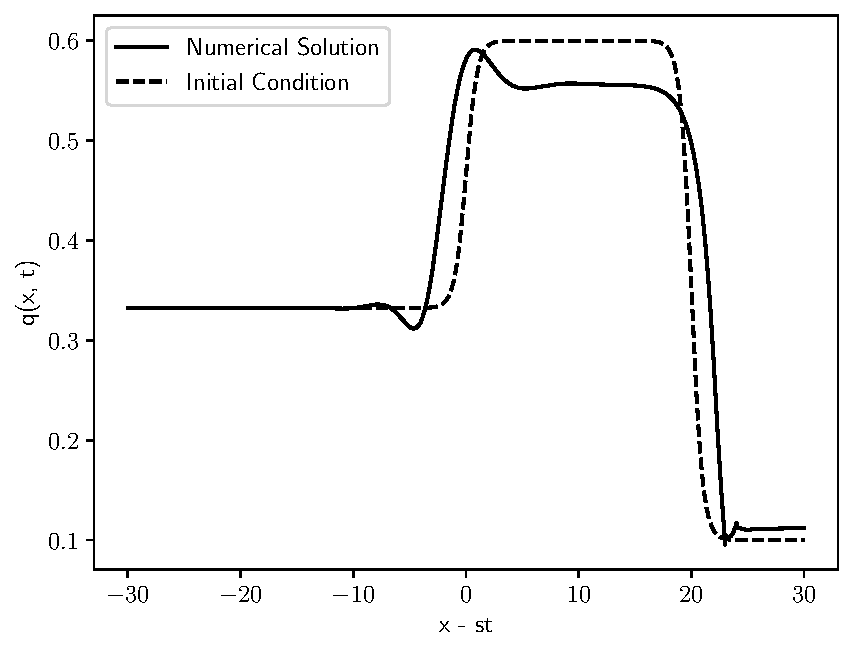
\includegraphics[scale=0.5]{figures/case_2_3.pdf}
    %   \caption{Case 2: Double Shock Structure}\label{fig:case2_3}
    % \end{figure}

  \subsubsection{Case 3: Undercompressive Double Shock}\label{sssec:case3}
    For the left state in the next regime, there is again a unique shock profile for all
    initial conditions.
    However this shock profile is not the single Lax shock seen in Case 1.
    With the following initial conditions,
    \begin{equation}
      q_0(x) = \p{\tanh{-x} + 1} \frac{q_l - q_r}{2} + q_r,
    \end{equation}
    where \(q_l = 0.4\) and \(q_r = 0.1\), Figure~\ref{fig:case3} shows a double shock
    structure.
    Similar to Figure~\ref{fig:case2} part (c), we see a undercompressive shock on the right
    and a Lax shock on the left.
    \begin{figure}
      \centering
      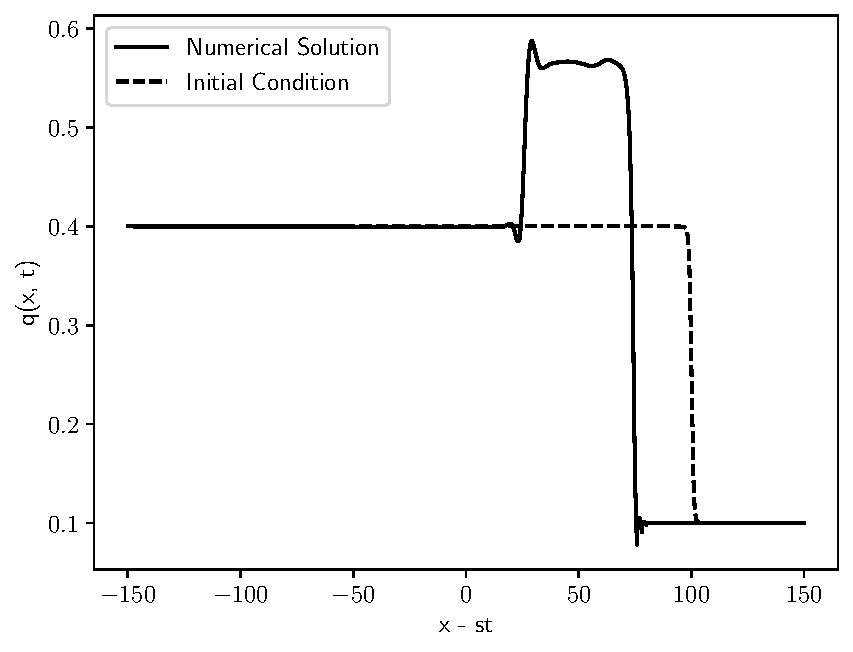
\includegraphics[scale=0.5]{figures/case_3_1.pdf}
      \caption{Case 3: Undercompressive Double Shock.}\label{fig:case3}
    \end{figure}

  \subsubsection{Case 4: Rarefaction-Undercompressive Shock}\label{sssec:case4}
    The final traveling wave structure appears when the left state is greater than the
    undercompressive shock height.
    In this case we see a rarefaction wave along with the undercompressive shock.
    Figure~\ref{fig:case4} shows the numerical solution for initial condition
    \begin{equation}
      q_0(x) = \p{\tanh{-x + 110} + 1} \frac{q_l - q_r}{2} + q_r,
    \end{equation}
    where \(q_l = 0.8\) and \(q_r = 0.1\).
    Note that the rarefaction wave and undercompressive shock are traveling at different
    speeds so they separate from each other.
    \begin{figure}
      \centering
      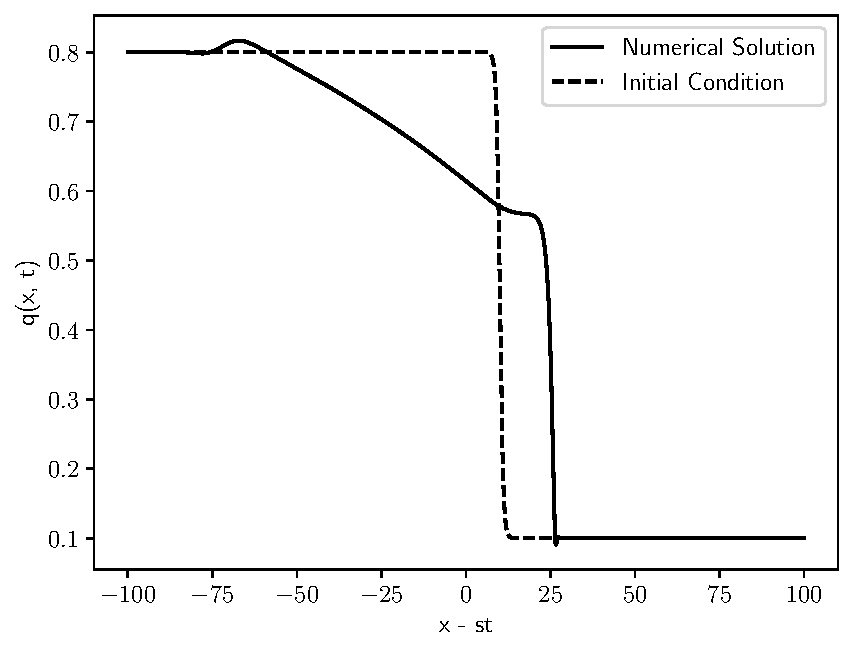
\includegraphics[scale=0.5]{figures/case_4_1.pdf}
      \caption{Case 4: Rarefaction-undercompressive shock.}\label{fig:case4}
    \end{figure}
